\section{UR3 Kinematics}

\subsection{Forward Kinematics} 

\noindent UR3 robot has a 6 joints as given in table \ref{tab:UR3_joints}.  

\begin{table}[htbp]
	\begin{center}
		\begin{tabular}{|c|c|c|}
			\hline
			%\cline{2-5} 
			\textbf{Movement axis} & \textbf{Working range} & \textbf{Maximum speed}\\
			\hline
			Base & $\pm 360\deg$ & $\pm 180\deg /sec$\\
			Shoulder & $\pm 360\deg$ & $\pm 180\deg /sec$\\
			Elbow & $\pm 360\deg$ & $\pm 180\deg /sec$ \\
			Wrist 1 & $\pm 360\deg$ & $\pm 180\deg/ sec$\\
			Wrist 2 & $\pm 360\deg$ & $\pm 180\deg /sec$\\
			Wrist 3 & infinite & $\pm 180\deg /sec$\\
			tool & - & $1m/sec$\\
			\hline
		\end{tabular}
		\caption{Joint details of the UR3 robot}
		\label{tab:UR3_joints}
	\end{center}
\end{table}

\noindent The Denavit-Hartenberg (DH) parameters of the UR3 robot are shown in the figure \ref{fig:DH} and DH values are given in the table \ref{tab:DH_values}. 

\begin{figure}[hbt!]
	\centering
	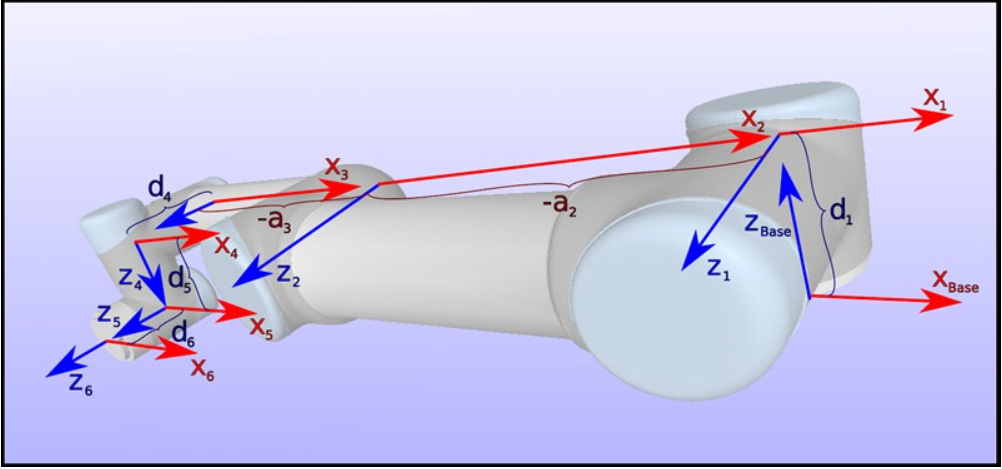
\includegraphics[scale=0.5]{DH.png}
	\caption{Denavit-Hartenberg (DH) parameters of the UR3} 
	\label{fig:DH}
\end{figure} 

\begin{table}[htbp]
	\begin{center}
		\begin{tabular}{|c|c|c|c|c|}
			\hline
			\cline{2-5} 
			\textbf{joint} & \textbf{\textit{$\theta_{i}$ [deg]}}& \textbf{\textit{$a_{i}$ [m]}}& \textbf{\textit{$d_{i}$ [m]}} & \textbf{\textit{$\alpha_{i}$ [deg]}}\\
			\hline
			i = 1& $\theta_{1}$& 0& 0.1519& 90 \\
			i = 2& $\theta_{2}$& -0.24356& 0& 0 \\
			i = 3& $\theta_{3}$& -0.21325& 0& 0 \\
			i = 4& $\theta_{4}$& 0& 0.11235& 90 \\
			i = 5& $\theta_{5}$& 0& 0.08535& -90 \\
			i = 6& $\theta_{6}$& 0& 0.0819& 0 \\
			\hline
		\end{tabular}
		\caption{DH parameters of the UR3 robot}
		\label{tab:DH_values}
	\end{center}
\end{table}

\noindent The transformation from joint $i$ to joint $i-1$ can be calculated by \ref{eq:transformation}, where $s_{\alpha_{i}}$ is the short form for $\sin(\alpha_{i})$ and $c_{\alpha_{i}}$ is the short form for $\cos(\alpha_{i})$
\begin{equation}
{}^{i}{T}_{i-1} = \left( \begin{array}{rrrr}                                
c_{\theta_{i}} & -c_{\theta_{i}} \cdot s_{\theta_{i}} & s_{\alpha_{i}} \cdot s_{\theta_{i}} & a_{i} \cdot c_{\theta_{i}} \\                                               
s_{\theta_{i}} & c_{\alpha_{i}} \cdot c_{\theta_{i}} & -s_{\alpha_{i}} \cdot c_{\theta_{i}} &  a_{i} \cdot s_{\theta_{i}} \\                                               
0 & s_{\alpha_{i}} & c_{\alpha_{i}} & d_{i} \\
0 & 0 & 0 & 1 \\                                               
\end{array}\right)
\label{eq:transformation}
\end{equation}

\noindent Forward kinematics of the UR3 robot can be calculated Using \ref{eq:transformation} as,  
\begin{equation*}
\tfMat{0}{T}{6} =\tfMat{0}{T}{1} \cdot \tfMat{1}{T}{2} \cdot \tfMat{2}{T}{3} \cdot \tfMat{3}{T}{4} \cdot \tfMat{4}{T}{5} \cdot \tfMat{5}{T}{6}
\end{equation*}

\subsection{Inverse Kinematics}
Inverse kinematics of UR3 robot can be solved analytically as per \cite{andersen2018kinematics}. However, there are 8 possible solutions based on the sign of the joint angles $\theta_{1}$, $\theta_{3}$, and $\theta_{5}$. This can be easily seen by considering the effect of the joint angle $\theta_{1}$ on $\theta_{5}$ as shown below.

\begin{equation*}
\theta_{5}=\pm \arccos\left(\frac{{}^{0}{P}_{6x} \cdot \sin(\theta_{1})-{}^{0}{P}_{6y} \cdot \cos(\theta_{1})-d_{4}}{d_{6}}\right)
\end{equation*}

\subsection{MoveIt configuration}

The primary objective of configuring the MoveIt is to generate semantic Robot Description Language (SRDF) \cite{SRDF} along with other important files needed to exploit MoveIt's capabilities. The important steps (not all of them) involved are given a brief introduction below.

\subsubsection{Self-Collision matrix} MoveIt checks if there is a possibility of collision between parts of the robot and this takes away the computation time. however, generating a self-collision matrix defines the pairs of links on the robot which are always in contact thus disabling these pairs from collision checking. Also, it defines the pairs which are never in contact so these also can be eliminated from collision checking.  

Since the phantom head is mounted to the robot's end-effector, it is necessary to account for collision checking. We roughly modeled the phantom head and added it to the URDF of the robot.

\begin{figure}[hbt!]
	\centering
	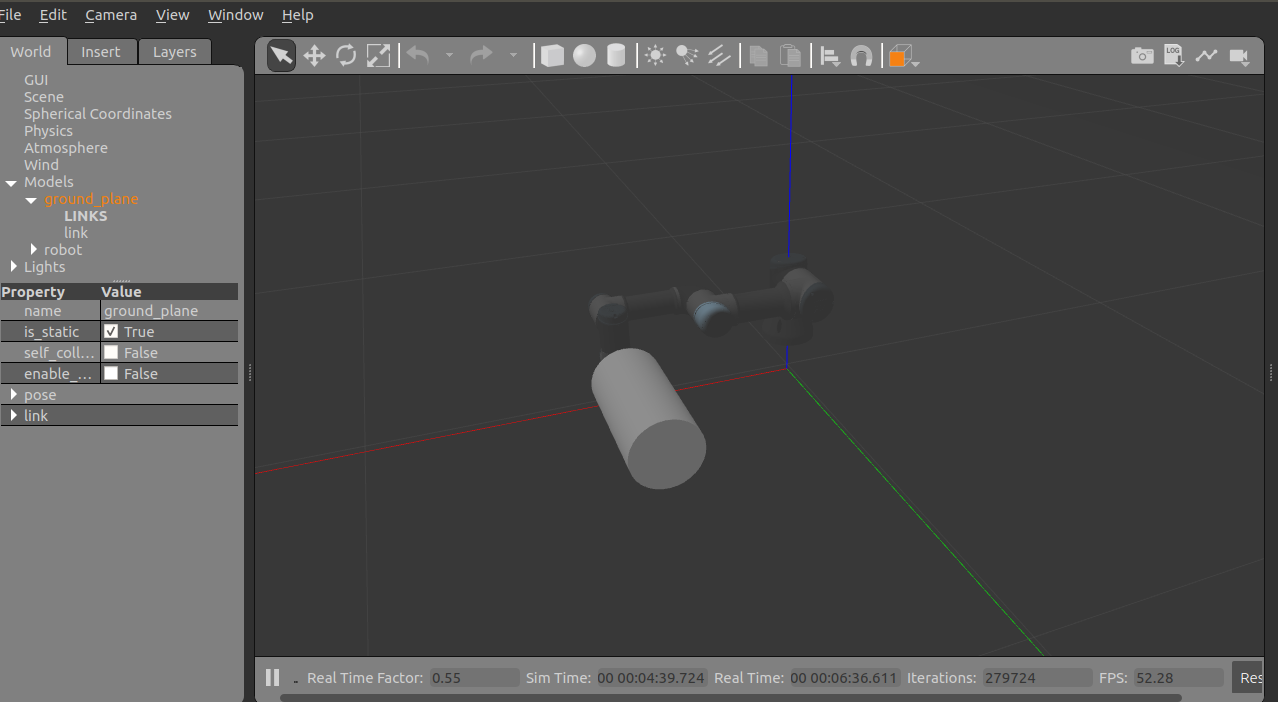
\includegraphics[width=\linewidth]{moveIt_phantom.png}
	\caption{Rough phantom model included in the robots URDF} 
	\label{fig:moveIt_phantom}
\end{figure}

\subsubsection{Virtual joints} Virtual joint attach the robot to the world therefore it is important to define it. Joint type and parent joint must be defined to create a virtual joint.

\subsubsection{Planning groups} Planning groups define the robot kinematic chain semantically and these groups are used later to move the robot. Appropriate kinematic solver has to be defined at this point to let MoveIt know which kinematic solver needs to be used. Popular choices are KDL, universal kinematics, or more powerful IK solver.

\subsubsection{Robot poses} We can define any fixed robot poses, for example, Home, later robot can be commanded to this position using inbuilt commands.

Moveit configuration package can be generated after completing a few more steps that are not discussed here. MoveIt offers many advantages when it comes to commanding the robot such as, 

\begin{enumerate}
	\item \textbf{Getting basic info} basic information such as end-effector position, move group details, planning frame, end-effector link, and joint states can be easily queried using MoveIt.
	\item \textbf{joint pose goal} robot can be commanded to a specific joint goal by defining an array of joint values.
	\item \textbf{pose goal} robot can be commanded to a specific pose by defining a homogeneous $4\times4$ pose matrix.
	\item \textbf{cartesian goal} robot can be commanded to follow a cartesian path by defining a list of waypoints for end-effector to go through.
	\item \textbf{trajectory display} we can visualize the path planned for the robot via any of the commanding methods.
	\item \textbf{Rviz \& Gazebo simulation} MoveIt seamlessly integrates Rviz and Gazebo simulation to enhance visualization.
\end{enumerate} 
